\chapter{Topic e LLM}

\section{Topic Modelling}

Per questa esercitazione si è scelto di usare il dataset \texttt{zou-lab/MedCaseReasoning} di \textit{Hugging Face} che contiene 14.489 righe di dati contenenti articoli medici. Osservando il grafico prodotto (fig. \ref{fig:1}) si può notare una coerenza semantica tra le keywords:

\begin{itemize}
  \item Il topic 0 sembra riferirsi a malattie cardiache (tachycardia, cardiomyopathy,heart). 
  \item Il topic 1 a malattie del sistema nervoso (encephalopathy, meningitis, encephalitis). 
  \item etc.
\end{itemize}

\begin{figure}[h]
    \centering
    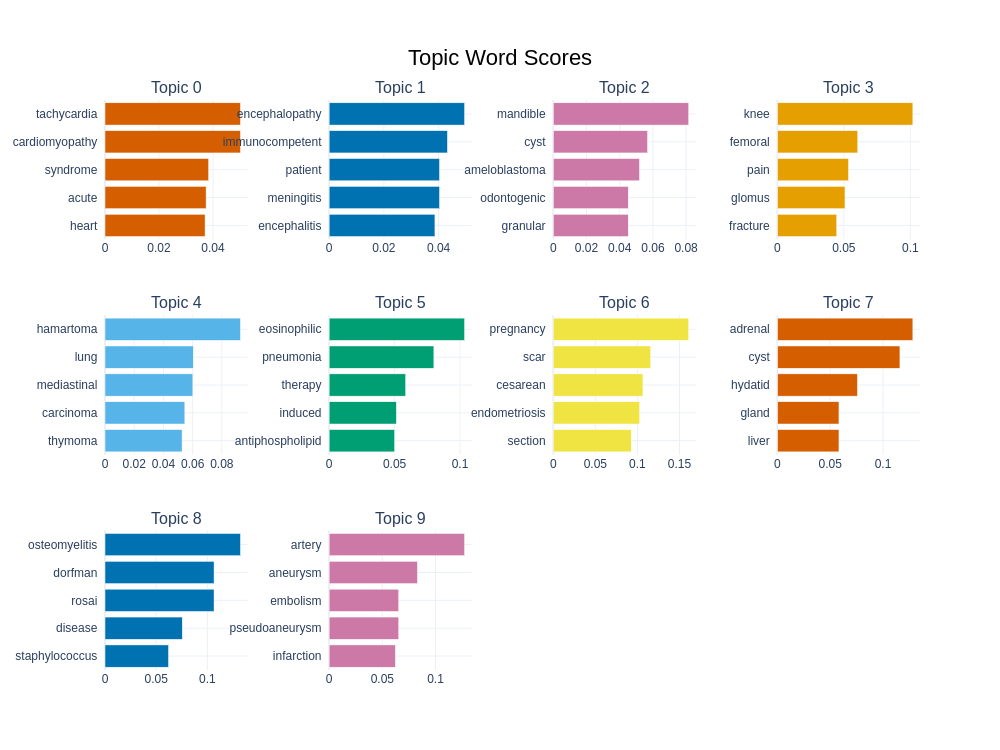
\includegraphics[scale=0.35]{newplot.png}
    \caption{Grafico a barre raffigurante i top topics.}
    \label{fig:1}
\end{figure}

\section{LLM Prompting}

In quest'ultima esercitazione si sono esplorate varie strategie di prompting e dei parametri dei modelli LLM.

\subsection{Label the Topic}

Il task consiste nell'assegnare un'etichetta ai topics prodotti nell'esercitazione precedente:

\begin{itemize}
  \item \textit{Zero-shot:} invece che assegnare una label ai topic assume che tutti i concetti appartengano a un unico paziente. 
  \item \textit{One-shot:} con un esempio il task diventa più preciso riuscendo a riassumere le caratteristiche comuni in un'unica etichetta.
\end{itemize}

\subsection{Guess from the Definitions}

Per tentare di far indovinare le parole dalla definizione si è utilizzato un approccio simile a quello usato per i topics: 

\begin{itemize}
  \item \textit{Zero-shot:} il modello fraintende il task assegnato e invece di restituire le parole restituisce una nuova definizione.
  \item \textit{One-shot:} aggiungendo un esempio sull'output atteso i risultati migliorano di molto. Il modello riesce a individuare correttamente le parole \textit{microscopio} e \textit{pericolo}, mentre è troppo generico su \textit{pantalone} (tenta con indumento) ed \textit{euristica} (linee guida).
  \item \textit{One-shot with suggestions:} aggiungendo al prompt precedente dei "suggerimenti", ossia le definizioni prese dal vocabolario della Treccani, si nota un miglioramento per la parola \textit{pantalone} che adesso viene riconosciuta correttamente più spesso. Per quanto riguarda \textit{euristica} viene restituito metodologia. 
\end{itemize}
